\chapter{Experiments}

\section{Overview}
\begin{itemize}
    \item Why transfer learning based approach ?
    \item Why classification ?
    \item Final goal of assessing stereotypical social bias in arguments produced by args.me search engine
\end{itemize}

Steps: 
\begin{enumerate}
    \item Collecting stereotypical samples with respect to different domains such as race, gender, profession etc. are gathered from the available sources (CrowS-Pairs \cite{nangia2020crows}, Social bias frames \cite{sap2019social}, StereoSet \cite{nadeem2020stereoset} as seen so far).
    \item Exploratory data analysis for some insights into the different types of biases (gender, race, profession, religion).
    \item Stereotypical dataset target labels interpretation
        \begin{itemize}
            \item Different perspectives of classification labels used 
            \item Anti-stereotypical samples introduced to get the perspective whether a text sequence is socially shared or not socially shared, as stereotypes can be interpreted as pictures in head.
            \item  Including unrelated as a category in classification, why?
        \end{itemize}
    \item Categorization experiments
    \begin{itemize}
        \item Binary classification 
        \item Multi-class classification 
        \item Multi-label classification 
        \item Why going with multi-label ?? When considering anti-stereotypical 
    \end{itemize}
\end{enumerate}
\section{Experimental setup}
\begin{itemize}
    \item Libraries used {Ktrain, huggingface, pytorch lightening}
    \item Classification head and the underlying methodology of transfer learning 
    \item Hyper-parameter search {RayTune}, search space
\end{itemize}
\section{Assessing stereotypical social bias}
\subsection{End-to-end Deep learning approach}
\begin{itemize}
    \item Brief description of language models with main underlying features
    
    Language models :
    \begin{itemize}
        \item GPT-2 \cite{radford2019language}
        
            Features :
    \begin{itemize}
        \item Training data 
        \item Training procedure
        \begin{itemize}
            \item Pre-processing
            \item pre-training
        \end{itemize}
        \item encoded stereotypes (research from stereoset and crows pair)
    \end{itemize}
        \item BERT-base-uncased
        
            Features \cite{devlin2018bert}:
            \begin{itemize}
                \item Training data : BookCorpus (11,038 unpublished books) and English Wikipedia text articles  
                \item Training procedure
                \begin{itemize}
                    \item Pre-processing : Lowercased, tokenized using wordpiece and vocab of size 30,000
                \item pre-training 
                \end{itemize}
                \item encoded stereotypes (research from stereoset and crows pair)
    \end{itemize}
        \item RoBERTa \cite{liu2019roberta}
        
            Features :
            \begin{itemize}
                \item Training data 
                \item Training procedure
                \begin{itemize}
                    \item Pre-processing
                    \item pre-training
                \end{itemize}
                \item encoded stereotypes (research from stereoset and crows pair)
            \end{itemize}
        \item XLnet \cite{yang2019xlnet}
        
            Features :
            \begin{itemize}
                \item Training data 
                \item Training procedure
                \begin{itemize}
                    \item Pre-processing
                    \item pre-training
                \end{itemize}
                \item encoded stereotypes (research from stereo-set and crows pair)
            \end{itemize}
    \end{itemize}
    \item Why these language model?
    \item Training process
        \begin{itemize}
            \item Basic architecture of huggingface transformer models for sequence classification consists of 3 modules, namely, transformer module (pre-trained language model with weights), dropout (layer normalization), classifier (target specific layer). 
            \item  Doing hyper-parameter search using the RayTune \footnote{\url{https://docs.ray.io/en/master/tune/index.html}} a python library for experiment execution and hyper-parameter tuning with the described model with classification head attached. Model hyperparameters can be defined as the parameters used to control the learning process which is set before training a model. \cite{bergstra2012random}\textbf{add reference}.  The goal of hyper-parameter search/optimization is to find optimal parameters out of search space. The three important features of hyper-parameter search are defining search space, defining search algorithm which is used to select the hyper-parameters from the search space and finally a metric which is used to evaluate the model with the hyper-parameter. The search space used is defined below 
            \begin{itemize}
                \item Learning rate : tune.loguniform(1e-5, 5e-5)
                \item "num\_train\_epochs": tune.choice([2,3,5])
                \item "per\_device\_train\_batch\_size": tune.choice([8, 16, 32])
            \end{itemize}
            The search algorithm used is basicVarientGenerator of ray which uses random search and grid search as algorithms. The objective metric is to reduce the validation loss. The models are run for 5 trials which leads to following trials  
        \begin{figure}[h]
            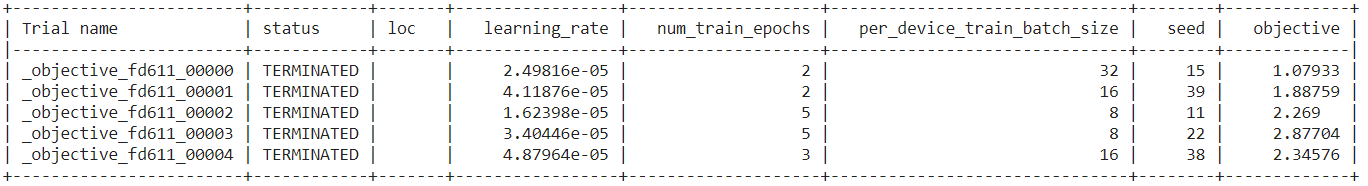
\includegraphics[width=12cm]{thesis/figures/hparameter.PNG}
            \centering
            \caption{Hyper-parameter search trails}
            \label{fig:The learning problem setup}
        \end{figure}
        
            \item Fine-tuning to target specific task (classification in our case) with target specific data (Multi-label dataset) by removing the language model head and replacing with 
            \begin{itemize}
                \item Linear layer with outputs corresponding to the number of labels 
                \item Adding corresponding activation function and loss function. As we are doing a multi label classification, we need to add a sigmoid activation function and binary cross entropy loss.
            \end{itemize}
        \item Training the fin-tuned model can be done by
        \begin{itemize}
            \item Training end - to - end wherein the entire fine-tuned model is trained and the loss is back-propagated to the entire network.
            \item Adaptive training where some layers of the initial layer of  pre-trained language model are freezed and the final layer of pre-trained model along with the attached classification head is trained. 
            \item Freezing the entire pre-trained model and only training the classification head attached. In this case only the  weights of the classification head are updated. 
        \end{itemize}
            
        \end{itemize}
\end{itemize}
\subsection{Baselines}

Questions:

\begin{enumerate}
    \item How does accuracy vary with non-contextual word embeddings (e.g. Glove, Word2Vec) to BERT word embedding?
    \item How does accuracy vary with baseline architecture (applying word embeddings to sentence and taking arithmetic average) to a fine-tuned BERT model ?
\end{enumerate}

    \begin{itemize}
        \item Lexicon - based approach : 
        \begin{itemize}
            \item Project into word embedding space and score each word based on its distance from woman, men ??
            \textbf{Refer }\cite{cryan2020detecting}
        \end{itemize}
        \item Brief description of  models and features
        \begin{itemize}
            \item SVM with selected lexicons + different features (toxicity, sentiment)
            \item Text-CNN with GLove,flair embedding
            \item Random embedding with GRU and LSTM 
        \end{itemize}
        \item Why these model?
    \end{itemize}
\section{Evaluation metrics} \cite{tsoumakas2007multi}
    \begin{itemize}
        \item Evaluation metrics selected for multi-label classification 
        \item Hamming loss 
        \item AUC-ROC score 
        \item Precision, recall, f-measure with respect to different categories
    \end{itemize}
    